% Chapter 4

\chapter{Nursing Care Dashboard (NCD)} % Write in your chapter title
\label{Chapter6}
\lhead{Chapter 6. \emph{Nursing Care Dashboard}} 
\section{NCD Perspective}
In this chapter, we provide a holistic perspective on the product highlighting its scope, functions, user classes, and architectural design to explain the vision and impact of the project within the healthcare domain.
The scope of ENS is focused on addressing the unique healthcare needs of elderly patients through a comprehensive set of functions. These functions encompass intelligent reporting, real-time monitoring, workflow integration, and AI-assisted insights. ENS seeks to enhance patient care, streamline workflows, reduce nurse burnout, and empower nurses and doctors with actionable insights. 
At the core of ENS is a user-centric approach to cater to the needs of nurses in the healthcare ecosystem. By prioritizing nurses, ENS aims to optimize user experience, facilitate collaboration, and improve patient outcomes. This emphasis on user classes and characteristics ensures that ENS is tailored to meet the specific requirements and preferences of the nurses.
The architectural framework of ENS highlights its technical sophistication and scalability. It uses different parts like cameras, AI in the cloud, and a website. This setup makes ENS a smart way to improve healthcare. It lets us easily collect, study, and share data. This lays the foundation for real-time patient monitoring and decision support. 
Beyond its immediate functionalities, ENS holds profound implications for the future of healthcare delivery.  ENS aims to revolutionize patient care by empowering healthcare professionals and enhancing the overall quality and efficiency of healthcare services. As we embark on this journey, we envision ENR as a catalyst for transformative change in the healthcare landscape, driving toward a future where nurses perform up to their potential and every patient receives personalized, proactive, and effective care.
 
\section{NCD Scope}
The scope of the product is defined in the following particulars:
\begin{itemize}
    \item The initial focus is on elderly patients
    \item Assist nursing care workflow
    \item Assist the doctor with decision and diagnosis
    \item Fixed number of activities and behaviors.
    \item The product will not detect abnormal activities.
    \item The product will be offered in home settings as well as in hospital settings
    \item The product will log vital signs with minimum human intervention.
    \item The product will alert the user in case of any irregularity in vital signs.
    \item Clients will be offered different payment and service plans.
\end{itemize}
\section{User Classes and Characteristics}
The most important users of the system are listed below in order of decreasing priority:
\begin{itemize}
    \item \textbf{Admin/Buyer:} For our business model the buyer of our product is the most important who will have the exclusive rights to maintain the whole system and the users associated with it.
    \item \textbf{Nurse:} The major user of the system around whom the whole system revolves. Some of their tasks will be automated while others digitized to remove anomalies produced in manual paperwork and management.
    \item \textbf{Doctor:} The decision maker. The doctor receives complete information about the patient from the nurse through the application. They can view the patient status, analyze near real-time data remotely, and make an informed decisions.
    \item \textbf{Caretaker:} The tertiary user of the system will only be able to view the patient status unless they are also the owner of the system.

\end{itemize}

Although the doctor makes the decisions, they rank below in priority as the system is aimed at assisting the nurses first. The Doctors' decision becomes secondary in a situation where there is no proper care being provided to the patient; where there is no proper patient information collection which is to be communicated to a doctor for decision making.
The caretakers need not have a screen but it is necessary to provide the caretakers of a patient the complete access to near real-time updates and status of their patient. This will allow them to rest easy in their home instead of staying in the hospitals for a long duration. It will also reduce the cynical attitude and delayed adoption of AI technology resulting in delayed technological advancements.
\pagebreak
\subsection{Database Diagram}
The Figure \ref{fig:db-diagram} shows the complete database that was utilized in the development of the prototype. The tables have been normalized to 3NF. Practically the patient logs are being kept in the InfluxDB Cloud to keep all the records while the rest of the database is in a single PostGreSql database deployed on NeonDB Cloud Serverless service.
\begin{figure}[h]
    \centering
    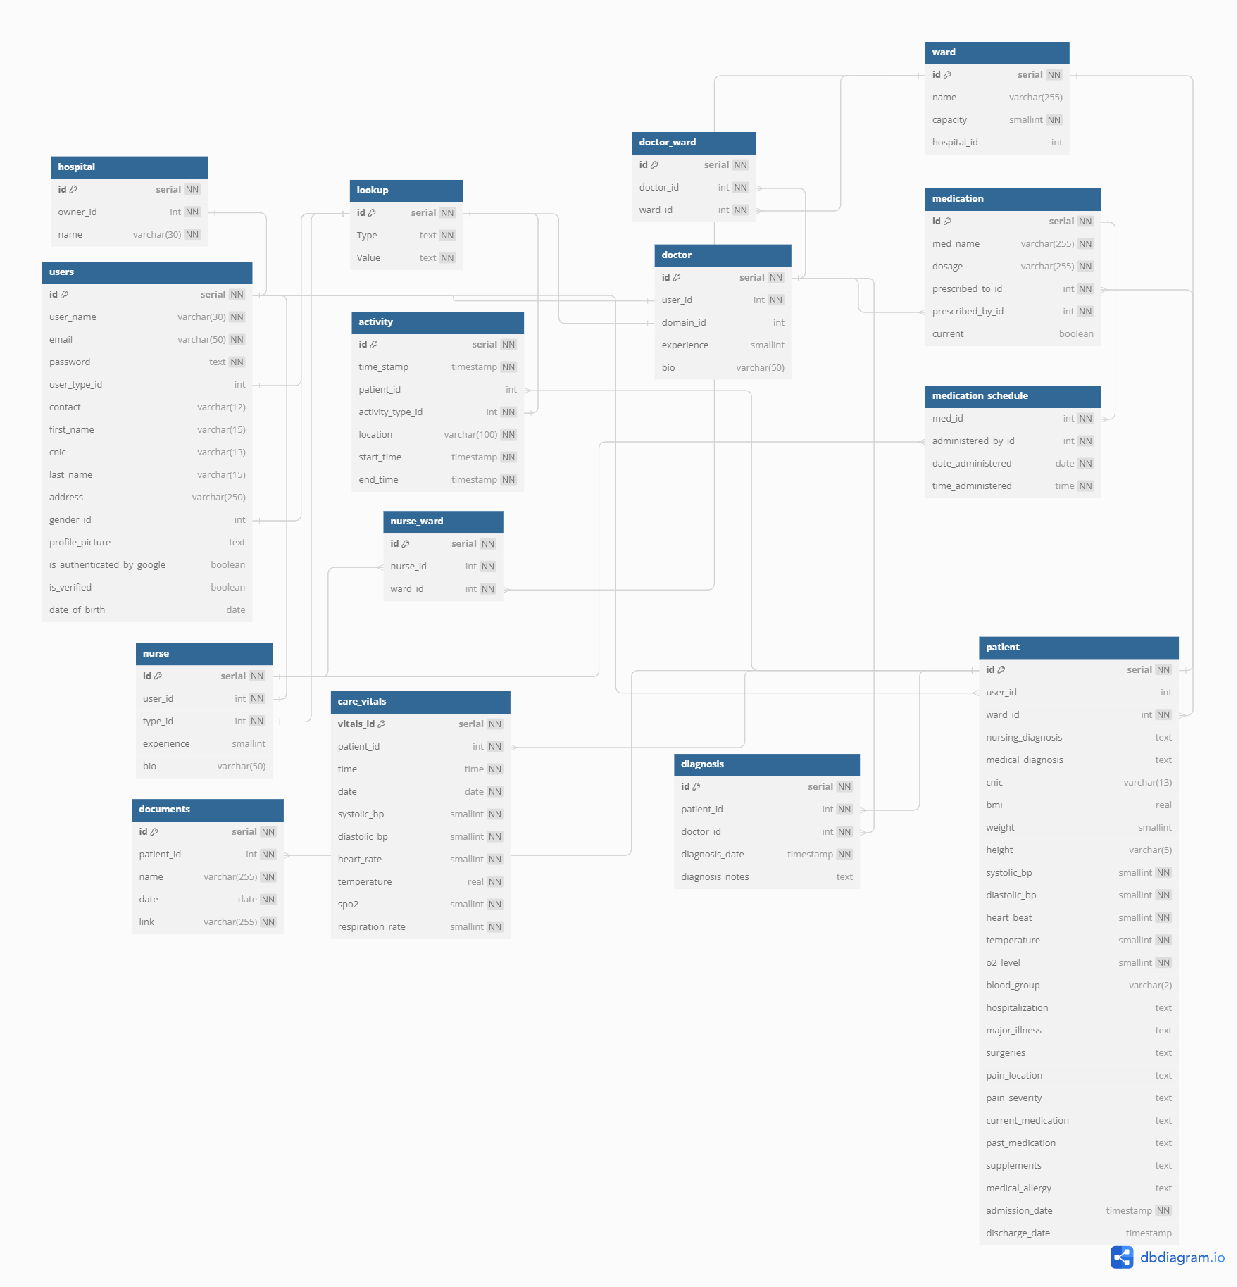
\includegraphics[width=\textwidth]{images/db.pdf}
    \caption{System Database Diagram}
    \label{fig:db-diagram}
\end{figure}
\section{Modules}
\subsection{Acquisition and Account}
\subsubsection{Purpose}
Authenticate users based on their credentials to allow only authorized users to view and manipulate sensitive patient records. It is also to allow authorized users to maintain and update their profiles as needed. Allow new payments to be processed and allow only authorized personnel to use the software in an attempt to curb software piracy. Moreover, to allow customers and potential clients to contact us. It is also aimed at improving the product based on feedback.
\subsubsection{Sub Modules}
\begin{enumerate}
    \item User Registration
    \item Account Management
    \item Payment Management
    \item Technical Support and Contact
\end{enumerate}
\subsubsection{Functional Requirements}
\begin{enumerate}
    \item      Hospital admin can sign up with a Google account or sign up with any email.
    \item Users are only allowed to login if they have been verified through email.
    \item Once verified they need to select a payment plan to proceed using the web portal.
    \item Hospital admin can add or remove doctors, nurses and patients.
    \item The users added by the hospital will be associated with the hospital.
    \item Hospital may choose existing doctor as well from a list of doctor accounts that are previously registered with the portal instead of making a duplicate account.
    \item The credentials will be auto-generated by the admin.
    \item The user may change their password after logging in successfully.
    \item Each user added by admin will be verified on login through an OTP sent to their mobile number.
    \item Users can view all payment plans offered.
    \item Users can select any of the payment plans of their choice.
    \item Users can make payment via an online payment gateway.
    \item Once payment is verified the user will receive a downloadable desktop application along with a unique product key.
    \item The user will be able to use the application if and only if they enter a valid product key.
    \item The user can renew their payment plan or change the plan if needed.
    \item Potential clients can navigate to the Contact Us page
    \item Potential clients can enter their details and a message in the contact form.
    \item Potential clients can use the Request Demo button to navigate to contact us page.
    \item Clients already using the product can send a feedback through their dashboard.
    \item Clients can also attach pictures of any bug they want to report.

\end{enumerate}

\subsection{Monitoring}
\subsubsection{Purpose}
Real-time monitoring and recording of vital signs, falls, sleeping patterns, and eating habits of aged patients.
\subsubsection{Sub Modules}
\begin{enumerate}
    \item Surveillance
    \item Push notification
    \item Logging and vital extraction
    \item real-time patient status
\end{enumerate}

\subsubsection{Functional Requirements}
\begin{enumerate}
    \item Vital signs monitoring using multiple cameras.
    \item Emergency detection in case of critical vitals of a patient.
    \item Object detection and tracking of patients.
    \item Generation of logs from monitoring.
    \item Processing, storing and analysis of logs.
    \item In case of missing readings and unknown activities, nurses or caretakers need to be prompted to enter information.
\end{enumerate}
The requirements for the doctor:
\begin{enumerate}
     \item Each vital and activity will be presented in tabular form with pagination available
     \item Doctor can apply ad-hoc queries to the data in the table.
     \item Data shall be represented in two different graphical forms:
    \begin{enumerate}
        \item One graph over a fixed duration of the previous 24 hours with anomalies marked.
        \item Second graph with user-defined duration to allow behavioural and statistical analysis of overall health condition.
    \end{enumerate}
    \item The doctor can also view the analysis produced by an AI model over any duration selected.
    \item The doctor can view the complete medical exam report generated by the nurse at the time of admittance.
    \item The doctor can also view previous medical records and reports entered into the system.
\end{enumerate}
For the Nurses:
\begin{enumerate}
    \item Latest vitals and activities of the patients in easy to read form.
    \item A graph over a fixed duration of the last hour.
    \item Patient data in form of reports and documentation entered into the portal.
\end{enumerate}
For the Caretakers:
\begin{enumerate}
    \item Complete history of medical records and reports.
    \item Complete patient exam at the time of admittance to a hospital.
    \item Real-time easy to read logs of vitals and activity.
    \item Graphical representation of each activity and vital with single line analysis of the latest health developments of patient provided by AI.
\end{enumerate}

\subsection{Nursing Care Automation}
\subsubsection{Purpose}
Aimed at automating and digitizing the nursing care process to reduce nurse workload and improve patient care. To provide better communication between the healthcare team. Provide easy to read and understand information about patient's health to the Doctors, Nurses and Caretakers.
\subsubsection{Sub Modules}
\begin{enumerate}
    \item Documentation (CRUD)
    \item Task Management
    \item Medication Management
\end{enumerate}
\subsubsection{Functional Requirements}
\begin{enumerate}
    \item Digitized nursing system for care planning, prioritization, and task management.
    \item Real-time statistics on patient health and status.
    \item Task reminders and decision support system for nurses.
    \item Easier documentation with predefined values and selections.
    \item Doctors can add notes to the patient report to communicate medicine, injection, or to conduct a medical test.
    \item Nurses add medication into the system to schedule reminders for dosage administration.
    \item Nurses and caretakers can upload the lab reports.
    \item Nurses can view the previously administered dosage allowing nurses from different shifts to stay up to date.
    \item Depending on location, hospital or home, the emergency alerts will be sent to nurses or to caretakers respectively.
    \item Alert is forwarded to another nurse if the first nurse didn't respond to an emergency in time.

\end{enumerate}
\section{Use Cases}
For the Use cases, the Table \ref{tab:use_cases} uses the following actors:
\begin{enumerate}
    \item Admin
    \item Doctor
    \item Nurse
    \item Caretaker
\end{enumerate}
When the table refers to All it means that all the actors can perform the task, but where the actor is listed as Any, it refers to any potential client that may or may not be a previous user of the system. The use case ID is in format x.y.z where x is the module number, y is the sub module and z is the use case number of that sub module.
\begin{longtable}{|p{2cm}|p{2.5cm}|p{2.5cm}|p{5cm}|}
    \caption{Use Case Table}
    \label{tab:use_cases} \\
    \hline
    UC Id & UC Name & Primary Actor & Functionality \\
    \hline
    \endfirsthead
    
    \multicolumn{4}{c}{\tablename\ \thetable\ -- \textit{Continued from previous page}} \\
    \hline
    UC Id & UC Name & Primary Actor & Functionality \\
    \hline
    \endhead
    
    \hline
    \multicolumn{4}{r}{\textit{Continued on next page}} \\
    \endfoot
    
    \hline
    \endlastfoot
        1.1.1 & Sign up  & Admin &  User can create an account\\
        \hline
        1.1.2 & Sign in   & All &  User can login to an existing account\\
        \hline
        1.1.3 & Add users  & Admin & User can register doctors, nurses, patients with the system.  \\
        \hline
        1.2.1 & Remove users & Admin & User can delete accounts of users associated with the hospital.\\
        \hline
        1.2.2 & Edit Profile & All & User can edit their PII\\
        \hline
        1.2.3 & Account Settings & All & User can manage their account settings\\
        \hline
        1.3.1 & Select Payment Plan & Admin & User can select and view payment and service plan of their choice.\\
        \hline
        1.3.2 & Online Payment  & Admin & User can make an online payment\\
        \hline
        1.3.3 & Update payment plan & Admin & User can update the payment plan\\
        \hline
        1.4.1 & Request a demo  & Any & User can request a demo of the product\\
        \hline
        1.4.2 & Provide Feedback & Nurse, Doctor, Caretaker & User can provide a feedback or report an error\\
        \hline
        1.4.3 & Request technical support & All & User can contact live support anytime\\
        \hline
        2.1.1 & AI model & Admin & User can select the AI model they want to run and view its output\\
        \hline
        2.2.1 & Alerts  & Nurse, Caretaker & User can view, respond and set  alerts \\
        \hline
        2.2.2 & Prompts for missing values & Nurse, Caretaker & User can enter the missing values\\
        \hline
         2.3.1 & Patient Status and Routine & Nurse, Caretaker& User can review patient vitals and activities in near realtime\\
        \hline
        2.3.2 & Infogra-phics  & Doctor, Caretaker & User can view graphs and analyze the patient health across various time periods.\\
        \hline
        2.3.3 & Patient Documents & Doctor, Caretaker, Nurse & User can view all previous documents of patient\\
        \hline
        3.1.1 & Document & Nurse & User can document the medical exam of patient and other necessary documents.\\
        \hline
         3.1.2 & Notes & Doctor, Nurse & User can add notes to patient file\\
        \hline
         3.1.3 & Upload Patient Reports & Nurse, Caretaker & User can upload patient report document\\
        \hline
        3.2.1 & Daily tasks & Nurse & User can view and manage daily tasks\\
        \hline
        3.3.1 & Update medication & Nurse, Caretaker & User can update the medication schedule of patient\\
        \hline
\end{longtable}
% \pagebreak
\section{Use Case Details}
\subsection{Sign Up}  

Use Case ID: 1.1.1\\ 
Pre Conditions: The user is on the sign up page.\\\
Post Conditions: User is successfully registered as an admin.\\\
Flow: 
\begin{enumerate}
    \item User enters their name, contact number, email, username, password and optionally their address. 
    \item User clicks on the sign up button to submit the information. 
    \begin{enumerate}
        \item If an account with the entered email already exists the user is informed to login instead
        \item If the account doesn't exists it continues from 3.
    \end{enumerate}
    \item The user receives an email which has a verification link redirecting the user to the webpage.
    \begin{enumerate}
        \item If the user opens the link within 24 hours the webpage shows a success dialog and redirects the user to login.
        \item If the link is not opened within 24 hours, the link expires and the webpage now shows a failure dialog.
    \end{enumerate}
\end{enumerate}
\subsection{Login} 
Use Case ID: 1.1.2\\\
Pre Conditions: The user is on the login page.\\\
Post Conditions: The user is succesfully logged into the portal\\\
Flow:
\begin{enumerate}
    \item User enters their username/email and password. 
    \item User presses enter button or clicks on the Login button to submit credentials
    \begin{enumerate}
        \item If the user exists and has his email verified then an OTP (One Time Password) is sent to the user's contact number.
        \begin{enumerate}
            \item IF the OTP is received, continue with step 3.
            \item If the OTP is not received the user can resend after a 60 seconds timer.
        \end{enumerate}
        \item If the user has signed up but the email is not verified then a dialog box appears informing users to verify the email first from their email inbox.
        \item If the user does not exist, a dialog box appears informing that the user doesn't exists.
    \end{enumerate}
    \item  User enters the OTP
    \begin{enumerate}
        \item If the user enters incorrect OTP then the user is prompted to re-enter the OTP.
        \item If the user enters correct OTP then he authenticates.
        \begin{enumerate}
            \item If the user hasn't selected a payment plan, the user gets redirected to a web page with payment plans available.
            \item If the user has selected and made a payment they can proceed to using the app.
        \end{enumerate}
    \end{enumerate}
\end{enumerate}
\subsection{User registration} 
Use Case ID: 1.1.3\\\
Pre Conditions: 
\begin{enumerate}
    \item Admin is logged into the web portal. 
    \item Admin has bought a subscription.
    \item Admin is on either of the "Doctors", "Nurses", "Patients" webpage.
\end{enumerate}
Post Conditions: 
\begin{enumerate}
    \item A user is registered and associated with the admin's hospital
    \item Registered user can login
\end{enumerate}
Flow: 
\begin{enumerate}
    \item The user clicks on the add button which pops up a dialog box with input fields
    \item The user enters the name, CNIC, contact, and age of the new user being registered.
    \begin{enumerate}
        \item If the user enters the name, CNIC, contact, and age in the wrong format then an alert is shown to correct the formats.
        \item If the user enters credentials with the correct format and:
        \begin{enumerate}
            \item If the user exists previously, then the new account is not created
            \item If the user does not exist previously, then the new account is created and we move to the next step.
        \end{enumerate}
    \end{enumerate}
    \item   A loading appears while the new user's password and username are auto generated.
    \item The generated credentials are emailed to the new user's email address.
\end{enumerate}
\subsection{Remove User} 
Use Case ID: 1.2.1\\\
Pre Conditions:
\begin{enumerate}
    \item Admin is logged into the web portal. 
    \item Admin has made a payment.
    \item Admin is on either of the "Doctors", "Nurses", "Patients" webpage.
\end{enumerate}
Post Conditions: The user of the system is removed \\\
Flow: 
\begin{enumerate}
    \item The user views a table with all the users available. 
    \item  User applies search filters to search the required user. 
    \item The user clicks on delete button to remove the user. 
    \item Alert dialog appears which asks to confirm deletion.
    \begin{enumerate}
        \item User clicks on "Delete" to remove the user.
        \item User clicks on "Cancel" which cancels the deletion process.
    \end{enumerate}
\end{enumerate}
\subsection{Edit Info} 
Use case id: 1.2.2\\\
Pre conditions:
\begin{enumerate}
    \item Admin is logged into the web portal. 
    \item Admin has made the payment and proceeds to the app.
    \item User is on "Edit Info" web page.
\end{enumerate}
Post conditions: User information is updated
Flow: 
\begin{enumerate}
    \item User clicks on the edit icon in the right corner of the information box.
    \item User has the option to edit the age, DOB, contact number, emergency contact, gender, address, and CNIC
    \item  Once done changing the values, the user presses the update button
    \begin{enumerate}
        \item User clicks on "Update" to update the information.
        \item User clicks on "Cancel" which cancels the updation process.
    \end{enumerate}
    
\end{enumerate}
\subsection{Account Settings} 
Use Case ID: 1.2.3\\\
Pre Conditions:
\begin{enumerate}
    \item Admin is logged into the web portal. 
    \item Admin has made the payment and proceeds to the app.
    \item Admin is on "Account Settings" web page.
\end{enumerate}
Post Conditions: User settings are updated\\\
Flow: 
\begin{enumerate}
    \item User scrolls down to update payment plan
    \begin{enumerate}
        \item User cancels the membership
        \begin{enumerate}
            \item A dialog box appears to confirm the cancellation
        \end{enumerate}
        \item The user changes the billing method
        \begin{enumerate}
            \item The user is redirected to payment gateway
        \end{enumerate}
    \end{enumerate}
    \item User clicks on deactivate or delete button
    \begin{enumerate}
        \item User is prompted to confirm the action
        \item User confirms or cancels the action
    \end{enumerate}
    \item User clicks on the edit icon
    \begin{enumerate}
        \item User changes the username, email or password.
    \item User enables or disables the 2FA (two factor authentication)
    \item User clicks on update
    \end{enumerate}
\end{enumerate}
\subsection{Payment and Service Plan} 
Use Case ID: 1.3.1\\\
Pre Conditions: None\\\
Post Conditions: None\\\
Flow: 
\begin{enumerate}
    \item User is logged in
    \begin{enumerate}
        \item User navigates to account settings
        \item User selects the "Change payment plan" option
        \item Continue
    \end{enumerate}
    \item New user visits the website and navigates to the payment plans
    \item Payment and Service plans offered are shown in card form
    \item User expands the cards for details for each
    \item User selects a payment plan of their choice .
    \begin{enumerate}
        \item If user is not logged in they are redirected to login page
    \end{enumerate}
    \item User is redirected to the payment gateway.
\end{enumerate}
\subsection{Online Payment} 
Use Case ID: 1.3.2\\\
Pre Conditions: User is logged in\\\
Post Conditions: Service is provisioned to the user\\\
Flow: 
\begin{enumerate}
    \item User selects the debit/credit card they want to use for payment
    \item User enter their card details
    \begin{enumerate}
        \item If the card details are correct then the user clicks on "Pay Now".
        \item Otherwise the user re-enters the card details.
    \end{enumerate}
    \item The user is prompted for a OTP that is received by them on their mobile phone.
    \item The user enters the OTP to complete the transaction.
    \item User receives an email of the receipt, link to downloading the desktop application and product licence key.
\end{enumerate}
\subsection{Update Payment Plan} 
Use Case ID: 1.3.3\\\
Pre Conditions: 
\begin{enumerate}
    \item User is logged in
    \item User is on Account Settings webpage
\end{enumerate}
Post Conditions: Payment Plan is Updated\\\
Flow: 
\begin{enumerate}
    \item The user checks the next billing date and changes their payment plan.
    \item When changing the payment plan they are redirected to payment gateway to re-enter their card information to confirm the update of service scheduled on from the next billing date.
    \item If user wants they can cancel their current plan to immediately shift to another plan. 
\end{enumerate}
\subsection{Request a demo} 
Use Case ID: 1.4.1\\\
Pre Conditions: None\\\
Post Conditions: None\\\
Flow: 
\begin{enumerate}
    \item User is on the product website
    \item User clicks on Request a demo button
    \item User is redirected to Contact Us webpage
    \item User enters their name, email and a short message
    \begin{enumerate}
        \item If the entered email, name, and message are not in the correct format then the user needs to correct it.
        \item Otherwise, user clicks on submit to send the request
    \end{enumerate}
\end{enumerate}
\subsection{Feedback} 
Use Case ID: 1.4.2\\\
Pre Conditions: User is logged in\\\
Post Conditions: None\\\
Flow: 
\begin{enumerate}
    \item User navigates to technical support page
    \item User selects the reason for contact from a drop-down menu.
    \item User enters the necessary details in the contact form.
    \item User adds images along text if needed in the contact form.
    \begin{enumerate}
        \item If the entered details are not in the correct format then the user needs to correct it.
        \item Otherwise, user clicks on submit to send the feedback.
    \end{enumerate}
\end{enumerate}
\subsection{Technical Support} 
Use Case ID: 1.4.3\\\
Pre Conditions: User is logged in\\\
Post Conditions: User is contacted with support staff\\\
Flow: 
\begin{enumerate}
    \item The user selects the Help \& Feedback tab from the dashboard which opens a page with a chat box in the left bottom.
    \item The user enters their issue in a chat box to which an online technical support staff responds in time. 
    \item If the issue cannot be resolved online, then a technical support member is sent to the user's location.
\end{enumerate}
\subsection{AI model} 
Use Case ID: 2.1.1\\\
Pre Conditions: 
\begin{enumerate}
    \item User is logged in
    \item Payment is verified
\end{enumerate}
Post Conditions:\\\
Flow:
\begin{enumerate}
    \item User selects the activity recognition model from a list of checkboxes. 
    \begin{enumerate}
        \item If an error occurs, an alert is popped up.
        \item Otherwise, the marked model(s) then run in real-time. 
    \end{enumerate}
    \item For each model, further options are available to select from such as specific activities, vitals or specific objects.
    \item Logs are generated, displayed on the desktop app, and sent to the cloud server for behaviour analysis. 
\end{enumerate}
\subsection{Alerts} 
Use Case ID: 2.2.1\\\
Pre Conditions: 
\begin{enumerate}
    \item User is logged in
    \item Alerts including emergency situations, missing values, communication messages and reminders notify the user with ring and vibration on the mobile app. 
\end{enumerate}
Post Conditions: None\\\
Flow: 
\begin{enumerate}
    \item The user opens the notification to respond appropriately in real-time. 
    \begin{enumerate}
        \item If the emergency situation is related to the vital signs, then the user has to provide suitable assistance to the patient, mark it as done.
        \item If alert is related to any missing vital, the user needs to add the vital sign manually.
        \item If the alert is related to a nursing task. Then the user needs to complete the task and mark it as done.
        \item If the alert is related to any object/activity that the AI models was not able to recognize, then the user needs to manually enter the data.
    \end{enumerate}
    \item User can tap on snooze button to snooze the alert for 5 minutes.
\end{enumerate}
\subsection{Prompt for missing values} 
Use Case ID: 2.2.2\\\
Pre Conditions: 
\begin{enumerate}
    \item User is logged in
    \item Alert due to a missing value is raised. 
\end{enumerate}
Post Conditions: The values are updated\\\
Flow: 
\begin{enumerate}
    \item The user is prompted to enter a missing value such as an unidentified object that is being consumed by a patient, or temperature readings. 
    \item The user enters the required value and submits the dialog box prompt.
    \begin{enumerate}
        \item If the entered value is not according to the right format/range then the user needs to re enter the value.
    \end{enumerate}
\end{enumerate}
\subsection{Patient Status and Routine} 
Use Case ID: 2.3.1\\\
Pre Conditions: 
\begin{enumerate}
    \item User is logged in
\end{enumerate}
Post Conditions: User is updated with any new developments about patient\\\
Flow:
\begin{enumerate}
    \item The user selects the All Patients tab from the sidebar. 
    \item The user searches the name of the patient from the table and then navigates to their profile to view complete routine of the patient.
    \item The routine shows the medication, eating, drinking and activities of the patient since 12am of that day.
    \item View any change of medicine or note attached by the doctor.
\end{enumerate}
\subsection{Infographics} 
Use Case ID: 2.3.2\\\
Pre Conditions: 
\begin{enumerate}
    \item User is logged in
\end{enumerate}
Post Conditions: User is updated with any new developments about patient\\\
Flow: 
\begin{enumerate}
    \item User navigates to a patient's tab to view data. 
    \item All the data is available in the form of graphs for the last hour. 
    \item User selects one of the graphs be it activity or a vital sign.
    \item The user is redirected to a page with in-depth analysis over the whole period of the patient for that specific health metric. 
    \item The user applies ad-hoc queries to filter and search through the tabular data as well as the info-graphic.
\end{enumerate}
\subsection{Patient Documents} 
Use Case ID: 2.3.3\\\
Pre Conditions: 
\begin{enumerate}
    \item User is logged in
\end{enumerate}
Post Conditions: User is able to download and view the required report\\\
Flow:
\begin{enumerate}
    \item User navigates to the Patient Documents to view all the previous medical records that are associated with that patient. 
    \item The user can apply filter to the reports. 
    \item The user can view complete medical history on a 3d model by selecting the year from the timeline dating back to the age of the user, on the left side of the 3d model.
\end{enumerate}
\subsection{Documentation} 
Use Case ID: 3.1.1\\\
Pre Conditions:
\begin{enumerate}
    \item User is logged in
    \item User is on the patient's document tab
\end{enumerate}
Post Conditions: Patient information is saved in the system\\\
Flow: 
\begin{enumerate}
    \item User opens the medical exam document tab. 
    \item User conducts the physical exam and documents the recordings in the form provided in the app.
    \item User presses submit to save the values
\end{enumerate}
\subsection{Notes} 
Use Case ID: 3.1.2\\\
Pre Conditions:
\begin{enumerate}
    \item User is logged in
    \item User is on the patient's documents tab
\end{enumerate}
Post Conditions: None\\\
Flow:
\begin{enumerate}
    \item The user clicks on the sticky note on the e-document that shows an "Add note" option. 
    \item User clicks on the option to attach a note to the patient file. 
    \item The user clicks on the sticky note on the e-document that shows a "View note" option. 
    \item User clicks on the option to view all previous notes to attached to the patient file.
\end{enumerate}
\subsection{Upload Patient Reports} 
Use Case ID: 3.1.3\\\
Pre Conditions: User is logged in\\\
Post Conditions: Patient report is readily available for the other users to download and view\\\
Flow: 
\begin{enumerate}
    \item The user navigates to Patient Exam tab to upload a lab test report. 
    \item The user selects the option Upload Report. The user selects either "Select from Gallery" or "Take a Picture" option. 
    \item User selects or takes an image and uploads it for the doctor to view.
\end{enumerate}
\subsection{Daily tasks} 
Use Case ID: 3.2.1\\\
Pre Conditions: User is logged in\\\
Post Conditions: None\\\
Flow: 
\begin{enumerate}
    \item The user views the tasks from a notification panel where the tasks are listed in order of highest priority first. 
    \item After completing the task, the user marks them as done. 
    \item The list gets updated when there is a change in schedule.
\end{enumerate}
\subsection{Update Medication} 
Use Case ID: 3.3.1\\\
Pre Conditions: User is logged in\\\
Post Conditions:\\\
Flow:
\begin{enumerate}
    \item User navigates to patient medication tab
    \item User add the required medication schedule
    \item User updates any current medication schedules if needed
    \item The duration of the patient medication is also then set to generate reminders for the user.
\end{enumerate}

\section{Risk Analysis}
Every project comes with risks of their own. Below are some of the risks involved in the project.
\subsection{Risks of the Project}
\begin{enumerate}
        \item The project stores sensitive patient information, raising concerns about data privacy and security. There is a risk of data breach or unauthorized access, which can lead to serious consequences. 
        \item The project uses AI models for activity recognition and forecasting. The models need to be trained enough to provide accurate results, otherwise nursing activities and patient health will be at risk.
        \item Our project requires interoperability with existing healthcare systems and technology. Incompatible systems may lead to inconsistency in patient data which will result in errors in patient care.
        \item Our project involves a significant investment of funds. There is a possibility that it will fail to produce the expected return on investment or fail to remain within the allocated budget.
        \item Our project might be exposed to internet-based attacks such as hacking or DOS attacks. As a result, unauthorized access to patient's data, interruptions in healthcare services, and other serious consequences can occur.
        \item There is a risk that healthcare professionals may not be willing to adopt the new technology and change their workflows. This could lead to resistance to change and potentially impact the success of the project.
\end{enumerate}
\subsection{Risk Mitigation}
\begin{enumerate}
        \item The patient information will be kept in encrypted in AES 128-bit format so that in case of data loss, the information stays meaningless to the threat agent.
        \item Professional and secure practices of programming will be utilised conforming to industry standards and guidelines to maintain integrity of the source code, application as well as the patient data.
        \item Nurses and Doctors will be provided training to navigate across the UI. The UI will be made following usability guidelines and will be updated frequently upon feeback from customers. A 24/7 technical call support staff will also be made available
        \item There is a demanding need for a system to help the nurse care workflow. There are hospitals in collaboration and the team shall be kept focused using agile scrum and kanban development life cycle to keep delivering and updating the system all while following a strict project timeline.
\end{enumerate}
